\subsection{REFERENCIAS Y COBERTURA EFECTIVA}

\begingroup\footnotesize\setlength{\tabcolsep}{3pt}
\begin{longtable}{L{4.2cm}rrrrr}
\caption{Referencias FEM explícitas refinadas. Fuente: registros de la campaña.}\label{tab:explicit-fem}\\
\toprule
Caso & Niveles & Grados de libertad & $T_{\max}$, °C & $\Delta T_{\max}$, K & Balance, \pct{}\\
\midrule\endfirsthead
\toprule
Caso & Niveles & Grados de libertad & $T_{\max}$, °C & $\Delta T_{\max}$, K & Balance, \pct{}\\
\midrule\endhead
aras\_flat & 3 & 264969 & 50.058 & 0.00349 & 0.01045\\
coaxial\_angular & 3 & 152951 & 31.980 & 0.00005 & 0.02704\\
kim\_sand & 3 & 2802105 & 49.757 & 0.00013 & 0.00805\\
xlpe\_backfill & 3 & 97221 & 33.525 & 0.01617 & 0.00673\\
xlpe\_discrete\_layers & 3 & 97217 & 37.371 & 0.03491 & 0.00156\\
xlpe\_dry\_far & 3 & 97221 & 36.889 & 0.03382 & 0.00736\\
xlpe\_dry\_near & 3 & 97221 & 42.862 & 0.07832 & 0.00741\\
xlpe\_single & 3 & 97221 & 36.852 & 0.03377 & 0.00718\\
\bottomrule\end{longtable}\endgroup

Todas las comparaciones de las etapas A--D utilizan estas referencias de la misma formulación física. El refinamiento verifica también el cambio de campo por material. La cantidad de semillas no debe confundirse con el número de instalaciones independientes.

\subsection{ARQUITECTURA Y TAMAÑO}

\begingroup\footnotesize\setlength{\tabcolsep}{3pt}
\begin{longtable}{L{4.2cm}rrrrr}
\caption{Etapa A: comparación de todas las semillas de desarrollo. Fuente: elaboración propia.}\label{tab:explicit-A}\\
\toprule
Configuración & Parámetros & Aceptadas & RMSE med., K & \makecell{Error máx.\\$T_{\max}$, K} & Violación máxima\\
\midrule\endfirsthead
\toprule
Configuración & Parámetros & Aceptadas & RMSE med., K & \makecell{Error máx.\\$T_{\max}$, K} & Violación máxima\\
\midrule\endhead
fourier\_w16\_d2 & 2202 & 0/4 & 1.090 & 16.823 & 19.965\\
local\_w16\_d2 & 1690 & 0/4 & 0.957 & 16.789 & 203.622\\
mixed\_w16\_d2 & 1924 & 0/4 & 0.548 & 12.064 & 26.087\\
mixed\_w32\_d3 & 11668 & 0/4 & 0.598 & 12.445 & 25.740\\
multipole\_w16\_d2 & 1784 & 0/4 & 0.199 & 0.221 & 7.596\\
subdomain\_w16\_d2 & 1754 & 2/4 & 0.213 & 0.784 & 5.075\\
subdomain\_w16\_d3 & 3114 & 0/4 & 0.269 & 0.909 & 9.241\\
subdomain\_w32\_d3 & 11338 & 3/4 & 0.195 & 0.511 & 1.560\\
subdomain\_w8\_d2 & 562 & 0/4 & 0.274 & 0.908 & 9.397\\
\bottomrule\end{longtable}\endgroup

La regla registrada selecciona \texttt{subdomain\_w32\_d3}. La selección es provisional: ninguna candidata cumple en todos los problemas y semillas de la etapa. No se declara una red o receta mínima admisible.

La violación máxima es el mayor cociente entre una métrica de rechazo y su tolerancia; un valor mayor que uno identifica incumplimiento. Las medianas incluyen también los intentos rechazados. Los parámetros corresponden al mayor tamaño total entre los casos de la etapa.

\begingroup\footnotesize\setlength{\tabcolsep}{3pt}
\begin{longtable}{L{5.2cm}L{4cm}r}
\caption{Mayor restricción relativa de la etapa A, incluidos los intentos rechazados. Fuente: elaboración propia.}\label{tab:explicit-A-diagnosis}\\
\toprule
Configuración & Restricción dominante & Cociente\\
\midrule\endfirsthead
\toprule
Configuración & Restricción dominante & Cociente\\
\midrule\endhead
fourier\_w16\_d2 & Tmax & 19.965\\
local\_w16\_d2 & Salto T & 203.622\\
mixed\_w16\_d2 & Salto flujo & 26.087\\
mixed\_w32\_d3 & Salto flujo & 25.740\\
multipole\_w16\_d2 & Salto T & 7.596\\
subdomain\_w16\_d2 & Salto T & 5.075\\
subdomain\_w16\_d3 & Salto T & 9.241\\
subdomain\_w32\_d3 & Salto T & 1.560\\
subdomain\_w8\_d2 & Salto T & 9.397\\
\bottomrule\end{longtable}\endgroup

La restricción dominante identifica dónde se incumple más la tolerancia, no demuestra por sí sola la causa de optimización.

La formulación mixta añade variables y ecuaciones; su rechazo con este presupuesto no refuta su equivalencia física. La comparación de Fourier conserva frecuencias fijadas y no optimiza su espectro. La variante multipolar ensayada tampoco agota todas las bases posibles.

\subsection{COLOCACIONES Y LOCALIZACIÓN}

\begingroup\footnotesize\setlength{\tabcolsep}{3pt}
\begin{longtable}{L{4.2cm}rrrrr}
\caption{Etapa B: comparación de todas las semillas de desarrollo. Fuente: elaboración propia.}\label{tab:explicit-B}\\
\toprule
Configuración & Parámetros & Aceptadas & RMSE med., K & \makecell{Error máx.\\$T_{\max}$, K} & Violación máxima\\
\midrule\endfirsthead
\toprule
Configuración & Parámetros & Aceptadas & RMSE med., K & \makecell{Error máx.\\$T_{\max}$, K} & Violación máxima\\
\midrule\endhead
interface\_2x & 13612 & 2/4 & 0.420 & 1.886 & 7.022\\
mixed\_1x & 13612 & 2/4 & 0.360 & 0.590 & 6.365\\
mixed\_2x & 13612 & 2/4 & 0.347 & 0.623 & 5.048\\
mixed\_4x & 13612 & 2/4 & 0.411 & 0.803 & 6.527\\
residual\_2x & 13612 & 2/4 & 0.332 & 0.940 & 6.257\\
uniform\_2x & 13612 & 0/4 & 0.459 & 6.920 & 8.213\\
\bottomrule\end{longtable}\endgroup

La regla registrada selecciona \texttt{mixed\_2x}. La selección es provisional: ninguna candidata cumple en todos los problemas y semillas de la etapa. No se declara una red o receta mínima admisible.

La violación máxima es el mayor cociente entre una métrica de rechazo y su tolerancia; un valor mayor que uno identifica incumplimiento. Las medianas incluyen también los intentos rechazados. Los parámetros corresponden al mayor tamaño total entre los casos de la etapa.

\begingroup\footnotesize\setlength{\tabcolsep}{3pt}
\begin{longtable}{L{5.2cm}L{4cm}r}
\caption{Mayor restricción relativa de la etapa B, incluidos los intentos rechazados. Fuente: elaboración propia.}\label{tab:explicit-B-diagnosis}\\
\toprule
Configuración & Restricción dominante & Cociente\\
\midrule\endfirsthead
\toprule
Configuración & Restricción dominante & Cociente\\
\midrule\endhead
interface\_2x & Salto T & 7.022\\
mixed\_1x & Salto T & 6.365\\
mixed\_2x & Salto T & 5.048\\
mixed\_4x & Salto T & 6.527\\
residual\_2x & Salto T & 6.257\\
uniform\_2x & Tmax & 8.213\\
\bottomrule\end{longtable}\endgroup

La restricción dominante identifica dónde se incumple más la tolerancia, no demuestra por sí sola la causa de optimización.

Un balance integral pequeño puede coexistir con errores del campo o de las interfaces. La nube uniforme deja pocas muestras próximas al cable dentro de un suelo extenso; se evalúa su consecuencia mediante FEM, sin considerar suficiente una pérdida de entrenamiento pequeña.

\subsection{AJUSTE DE ENTRENAMIENTO}

\begingroup\footnotesize\setlength{\tabcolsep}{3pt}
\begin{longtable}{L{4.2cm}rrrrr}
\caption{Etapa C: comparación de todas las semillas de desarrollo. Fuente: elaboración propia.}\label{tab:explicit-C}\\
\toprule
Configuración & Parámetros & Aceptadas & RMSE med., K & \makecell{Error máx.\\$T_{\max}$, K} & Violación máxima\\
\midrule\endfirsthead
\toprule
Configuración & Parámetros & Aceptadas & RMSE med., K & \makecell{Error máx.\\$T_{\max}$, K} & Violación máxima\\
\midrule\endhead
lr\_0.0005 & 13612 & 2/4 & 0.419 & 0.581 & 4.487\\
lr\_0.001 & 13612 & 1/4 & 0.377 & 0.602 & 4.424\\
lr\_0.002 & 13612 & 1/4 & 0.277 & 0.195 & 5.131\\
\bottomrule\end{longtable}\endgroup

La regla registrada selecciona \texttt{lr\_0.0005}. La selección es provisional: ninguna candidata cumple en todos los problemas y semillas de la etapa. No se declara una red o receta mínima admisible.

La violación máxima es el mayor cociente entre una métrica de rechazo y su tolerancia; un valor mayor que uno identifica incumplimiento. Las medianas incluyen también los intentos rechazados. Los parámetros corresponden al mayor tamaño total entre los casos de la etapa.

\subsection{CALIBRACIÓN ADICIONAL DE CONTINUIDAD TÉRMICA}

Esta ampliación se registró durante B, antes de C y de toda confirmación, al persistir saltos térmicos excesivos con refinamiento de puntos. Cambia únicamente el peso de continuidad de temperatura; conserva las ecuaciones, normalizaciones y tolerancias. El peso 100 reutiliza cuatro ejecuciones de C; 1000 y 10000 añaden ocho entrenamientos. Las corridas reutilizadas no se cuentan dos veces en el total.

\begingroup\footnotesize\setlength{\tabcolsep}{3pt}
\begin{longtable}{L{4.2cm}rrrrr}
\caption{Etapa C2: comparación de todas las semillas de desarrollo. Fuente: elaboración propia.}\label{tab:explicit-C2}\\
\toprule
Configuración & Parámetros & Aceptadas & RMSE med., K & \makecell{Error máx.\\$T_{\max}$, K} & Violación máxima\\
\midrule\endfirsthead
\toprule
Configuración & Parámetros & Aceptadas & RMSE med., K & \makecell{Error máx.\\$T_{\max}$, K} & Violación máxima\\
\midrule\endhead
weight\_100 & 13612 & 2/4 & 0.419 & 0.581 & 4.487\\
weight\_1000 & 13612 & 2/4 & 0.345 & 0.676 & 1.595\\
weight\_10000 & 13612 & 2/4 & 0.276 & 0.477 & 2.075\\
\bottomrule\end{longtable}\endgroup

La regla registrada selecciona \texttt{weight\_1000}. La selección es provisional: ninguna candidata cumple en todos los problemas y semillas de la etapa. No se declara una red o receta mínima admisible.

La violación máxima es el mayor cociente entre una métrica de rechazo y su tolerancia; un valor mayor que uno identifica incumplimiento. Las medianas incluyen también los intentos rechazados. Los parámetros corresponden al mayor tamaño total entre los casos de la etapa.

\subsection{MENOR RED POR PROBLEMA DENTRO DEL ESPACIO ENSAYADO}

\begingroup\footnotesize\setlength{\tabcolsep}{3pt}
\begin{longtable}{L{3.5cm}L{4.2cm}rr}
\caption{Menor red aceptada por problema entre las candidatas de A. No es una garantía fuera del caso ensayado. Fuente: elaboración propia.}\label{tab:explicit-smallest}\\
\toprule
Problema & Menor candidata & Parámetros & RMSE med., K\\
\midrule\endfirsthead
\toprule
Problema & Menor candidata & Parámetros & RMSE med., K\\
\midrule\endhead
coaxial\_angular & Ninguna & -- & --\\
xlpe\_single & subdomain\_w16\_d2 & 1754 & 0.381\\
\bottomrule\end{longtable}\endgroup

\subsection{INSENSIBILIDAD Y PRESUPUESTOS DE COLOCACIÓN}

\begingroup\footnotesize\setlength{\tabcolsep}{3pt}
\begin{longtable}{L{4.2cm}rrrr}
\caption{Colocaciones efectivas por problema y factor. Las interfaces tienen dos trazas en una misma posición. Fuente: elaboración propia.}\label{tab:explicit-point-counts}\\
\toprule
Caso & Factor & Interior suelo & Interior cable & Interfaces\\
\midrule\endfirsthead
\toprule
Caso & Factor & Interior suelo & Interior cable & Interfaces\\
\midrule\endhead
xlpe\_single & 1x & 256 & 512 & 384\\
xlpe\_single & 2x & 512 & 1024 & 768\\
xlpe\_single & 4x & 1024 & 2048 & 1536\\
xlpe\_discrete\_layers & 1x & 512 & 512 & 480\\
xlpe\_discrete\_layers & 2x & 1024 & 1024 & 960\\
xlpe\_discrete\_layers & 4x & 2048 & 2048 & 1920\\
\bottomrule\end{longtable}\endgroup

Las políticas uniforme, de interfaz y residual se comparan con el presupuesto 2x. Estos conteos excluyen las cuadraturas auxiliares: cada lado exterior emplea 96 veces el factor y cada conductor usa el máximo entre 256 y 128 veces el factor para la integral eléctrica, activa en DC. Por ello, el contraste 1x--4x aumenta el presupuesto espacial conjunto, no aísla solo los puntos interiores. No se interpreta la suma como una malla FEM ni se cuenta cada traza de interfaz como una posición nueva.

\begingroup\footnotesize\setlength{\tabcolsep}{3pt}
\begin{longtable}{L{4.2cm}rrrrr}
\caption{Insensibilidad observada al aumentar colocaciones. Ambos cálculos deben estar aceptados. Fuente: elaboración propia.}\label{tab:explicit-convergence}\\
\toprule
Caso & Semilla & Cambio & $D$, \pct{} & $H$, \pct{} & Insensible\\
\midrule\endfirsthead
\toprule
Caso & Semilla & Cambio & $D$, \pct{} & $H$, \pct{} & Insensible\\
\midrule\endhead
xlpe\_single & 11 & 1x--2x & 1.979 & 0.913 & No\\
xlpe\_single & 11 & 2x--4x & 1.904 & 1.790 & No\\
xlpe\_single & 23 & 1x--2x & 1.376 & 0.392 & No\\
xlpe\_single & 23 & 2x--4x & 2.261 & 2.915 & No\\
xlpe\_discrete\_layers & 11 & 1x--2x & 1.514 & 0.189 & No\\
xlpe\_discrete\_layers & 11 & 2x--4x & 0.457 & 0.732 & No\\
xlpe\_discrete\_layers & 23 & 1x--2x & 3.056 & 1.028 & No\\
xlpe\_discrete\_layers & 23 & 2x--4x & 1.770 & 1.756 & No\\
\bottomrule\end{longtable}\endgroup

Se cumple la comprobación de insensibilidad en 0 de 8 comparaciones. Las diferencias restantes impiden afirmar independencia universal del número de colocaciones.

Este contraste corresponde al presupuesto y pesos de B. El ajuste posterior de C y C2 no convierte retrospectivamente esos pares en convergentes ni demuestra independencia de colocaciones de la receta final. La aceptación de D se refiere a errores y criterios físicos evaluados frente a FEM con el presupuesto congelado.

\subsection{CONFIRMACIÓN CON SEMILLAS INDEPENDIENTES}

\begingroup\footnotesize\setlength{\tabcolsep}{3pt}
\begin{longtable}{L{3.4cm}rrrrr}
\caption{Confirmación de la receta congelada: semillas 71, 83 y 97. Fuente: elaboración propia.}\label{tab:explicit-production}\\
\toprule
Caso & Aceptadas & RMSE med., K & RMSE mín.--máx., K & \makecell{Error máx.\\$T_{\max}$, K} & Balance máx., \pct{}\\
\midrule\endfirsthead
\toprule
Caso & Aceptadas & RMSE med., K & RMSE mín.--máx., K & \makecell{Error máx.\\$T_{\max}$, K} & Balance máx., \pct{}\\
\midrule\endhead
aras\_flat & 0/3 & 1.707 & 1.696--2.632 & 8.321 & 0.237\\
kim\_sand & 0/3 & 1.690 & 1.625--2.495 & 8.558 & 2.680\\
xlpe\_backfill & 0/3 & 0.734 & 0.730--1.185 & 1.347 & 2.928\\
xlpe\_discrete\_layers & 0/3 & 0.301 & 0.163--0.474 & 0.797 & 1.046\\
xlpe\_dry\_far & 3/3 & 0.296 & 0.263--0.338 & 0.441 & 0.962\\
xlpe\_dry\_near & 1/3 & 0.733 & 0.499--0.746 & 2.474 & 1.717\\
xlpe\_single & 3/3 & 0.253 & 0.243--0.257 & 0.378 & 0.873\\
\bottomrule\end{longtable}\endgroup

Los casos aceptados parcialmente no se consideran configuraciones robustas. Ninguna semilla de confirmación se utilizó para elegir la receta de C y C2. Las diferencias de rendimiento entre casos corresponden a transferencia del procedimiento con reentrenamiento, no de una única red ya entrenada.

\begingroup\footnotesize\setlength{\tabcolsep}{3pt}
\begin{longtable}{L{4.2cm}rrr}
\caption{Efectos térmicos respecto al control XLPE homogéneo, a igual fuente prescrita. Fuente: elaboración propia.}\label{tab:explicit-effects}\\
\toprule
Escenario & $\Delta T^F_{\max}$, K & Mediana $\Delta T^P_{\max}$, K & Pares aceptados\\
\midrule\endfirsthead
\toprule
Escenario & $\Delta T^F_{\max}$, K & Mediana $\Delta T^P_{\max}$, K & Pares aceptados\\
\midrule\endhead
xlpe\_backfill & -3.327 & -4.080 & 0/3\\
xlpe\_dry\_near & 6.009 & 3.893 & 1/3\\
xlpe\_dry\_far & 0.036 & -0.089 & 3/3\\
xlpe\_discrete\_layers & 0.519 & 0.574 & 0/3\\
\bottomrule\end{longtable}\endgroup

Las diferencias FEM caracterizan los pares físicos; una diferencia PINN de un par rechazado es diagnóstica y no confirma el efecto mediante el artefacto. El control homogéneo utiliza k del suelo base, no se identifica automáticamente con un promedio equivalente del mapa heterogéneo.

\begingroup\footnotesize\setlength{\tabcolsep}{3pt}
\begin{longtable}{L{4.2cm}rrr}
\caption{Resolución empírica del efecto: discretización y variabilidad pareada. Fuente: elaboración propia.}\label{tab:explicit-effect-resolution}\\
\toprule
Caso & Cambio de malla, K & Rango PINN, K & Resuelto\\
\midrule\endfirsthead
\toprule
Caso & Cambio de malla, K & Rango PINN, K & Resuelto\\
\midrule\endhead
xlpe\_backfill & 0.01759 & 0.511 & No\\
xlpe\_dry\_near & 0.04455 & 1.854 & No\\
xlpe\_dry\_far & 0.00005 & 0.131 & No\\
xlpe\_discrete\_layers & 0.00114 & 0.814 & No\\
\bottomrule\end{longtable}\endgroup

Se exige aceptación de los tres pares, signos coincidentes con FEM y tanto rango PINN como cambio del efecto por malla menores que el módulo del efecto FEM. Esta regla se explicitó antes de D. Es una comprobación empírica de resolución, sin intervalos poblacionales ni cotas rigurosas de error.

La ubicación del máximo se conserva en el expediente sobre la nube común de conductores. El muestreo y la escasa diferencia térmica dentro del metal impiden atribuir precisión milimétrica a esa ubicación. OE3 dispone de temperaturas y efectos contrastados, pero no de una certificación del punto caliente continuo; no se confunde una máxima muestreada con una búsqueda espacial convergente.

\begin{figure}[p]\centering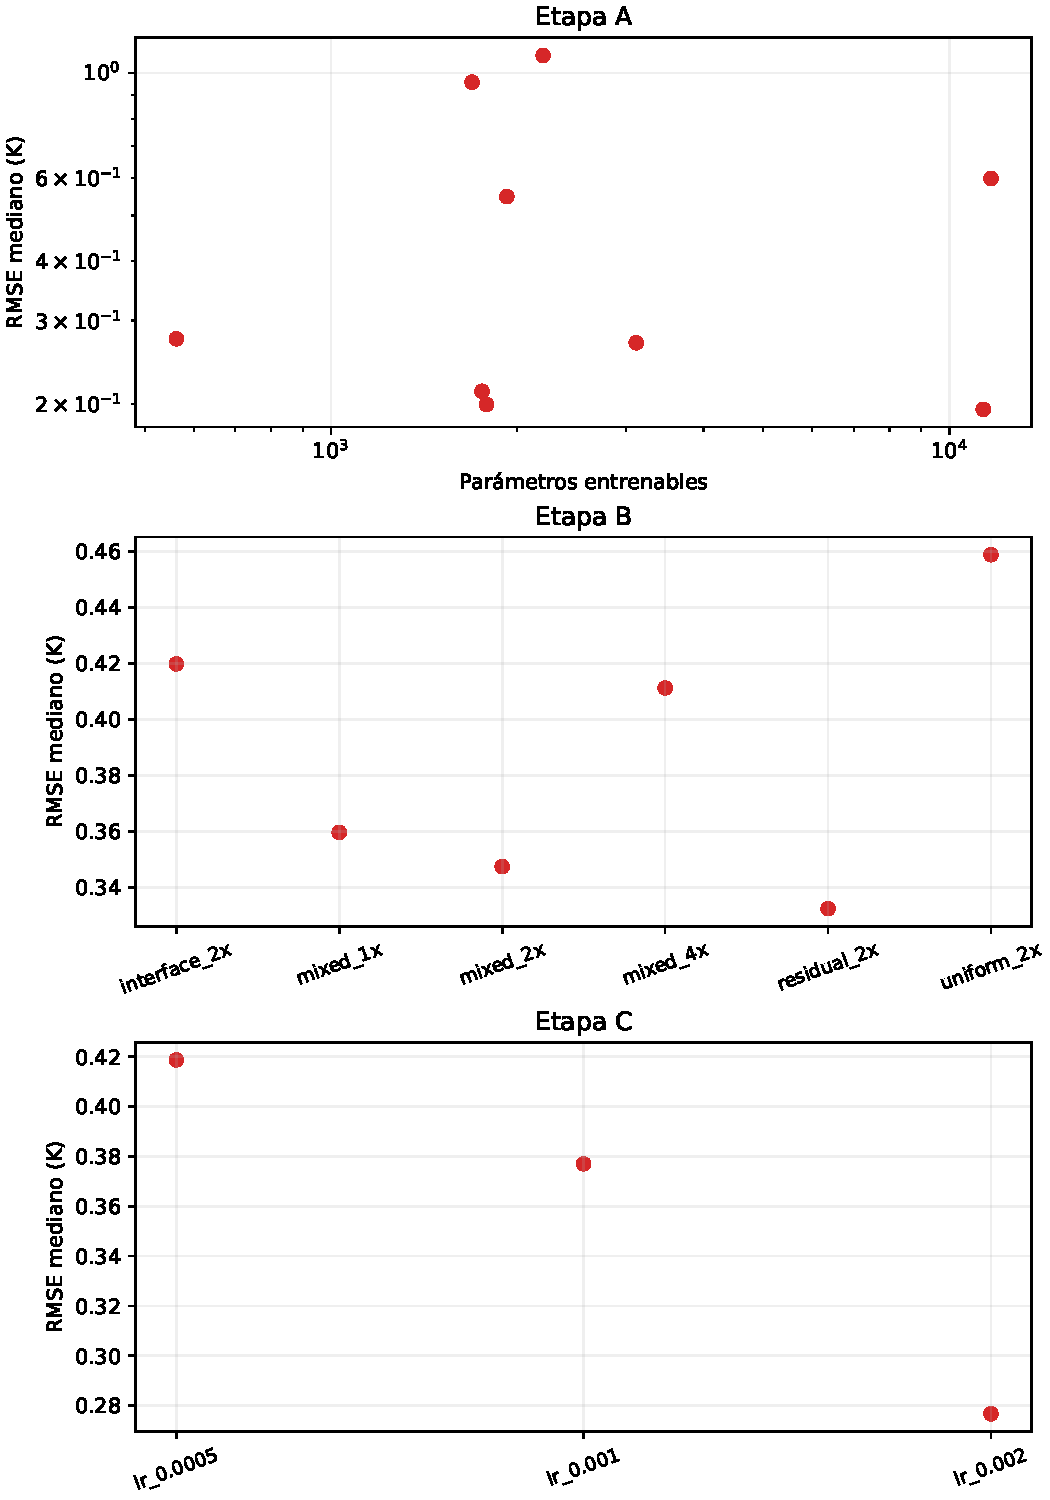
\includegraphics[width=.88\textwidth,height=.82\textheight,keepaspectratio]{explicit/selection.pdf}

\caption{Comparación de desarrollo. Verde: aceptación completa; rojo: al menos un rechazo. Los paneles corresponden a etapas distintas y no a un único factorial. Fuente: elaboración propia.}\end{figure}

\begin{figure}[htbp]\centering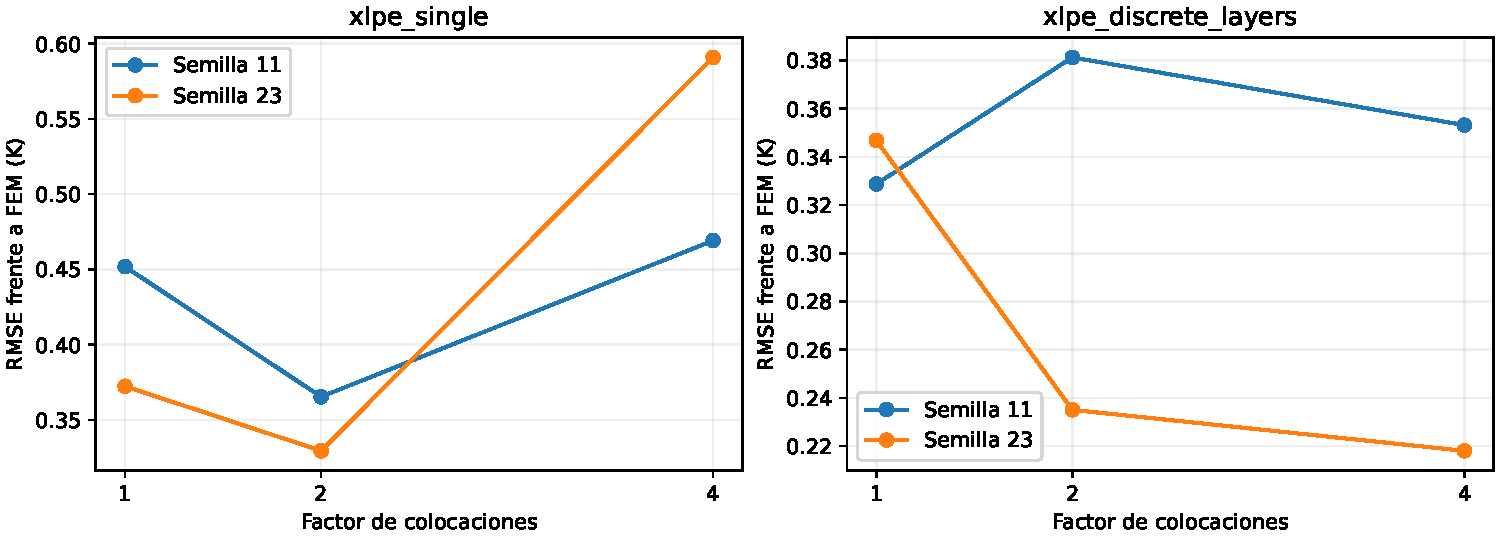
\includegraphics[width=\textwidth]{explicit/convergence.pdf}

\caption{Sensibilidad al número de colocaciones con la misma arquitectura y política geométrica. Fuente: elaboración propia.}\end{figure}

\begin{figure}[p]\centering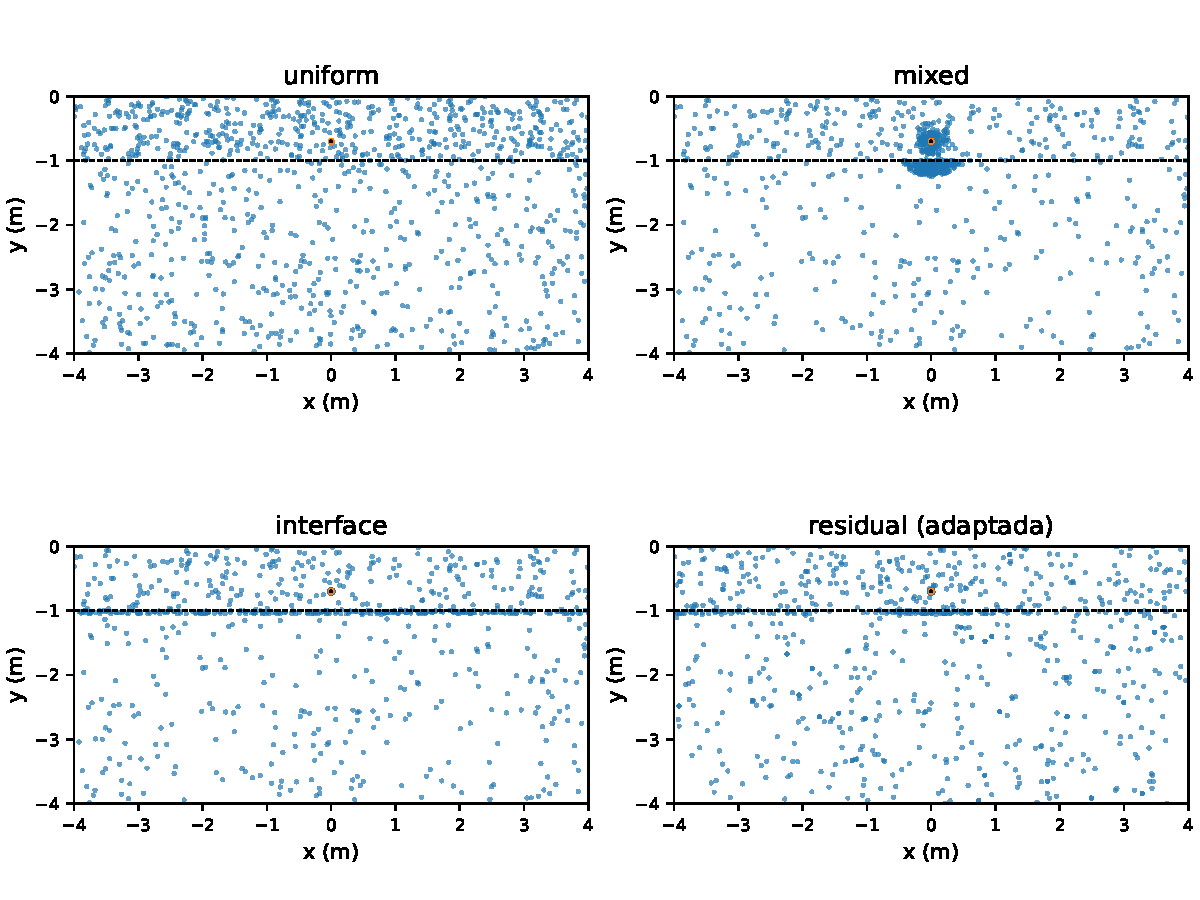
\includegraphics[width=\textwidth]{explicit/collocation_domain.pdf}

\caption{Cobertura del dominio para las cuatro políticas a igual presupuesto 2x, estratos y semilla 11. Azul: suelo; naranja: materiales del cable; líneas: interfaces geométricas. Se muestran colocaciones interiores, no las cuadraturas de trazas. Fuente: nubes archivadas; la política residual muestra la nube posterior a la adaptación.}\end{figure}

\begin{figure}[p]\centering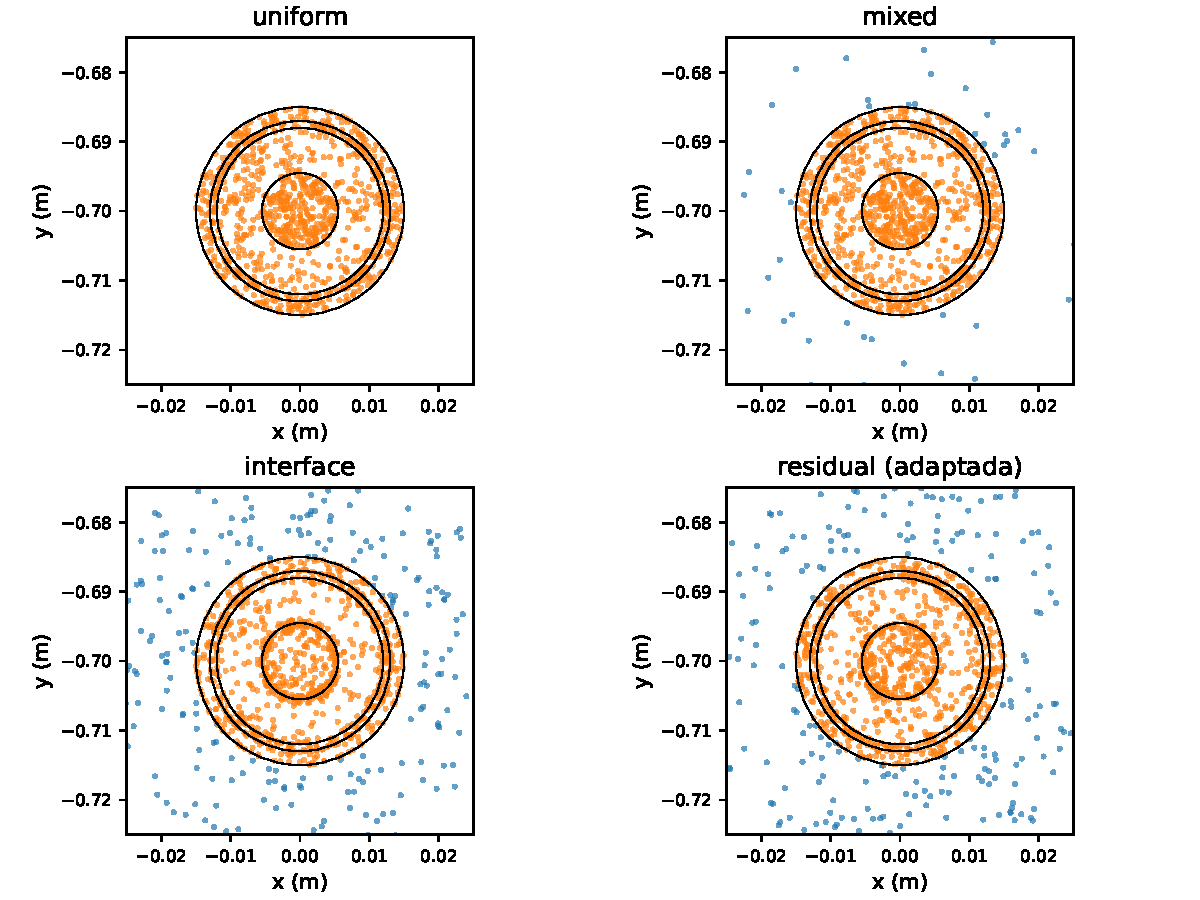
\includegraphics[width=\textwidth]{explicit/collocation_detail.pdf}

\caption{Detalle del cable para las cuatro políticas a igual presupuesto 2x, estratos y semilla 11. Azul: suelo; naranja: materiales del cable; líneas: interfaces geométricas. Se muestran colocaciones interiores, no las cuadraturas de trazas. Fuente: nubes archivadas; la política residual muestra la nube posterior a la adaptación.}\end{figure}

\begin{figure}[htbp]\centering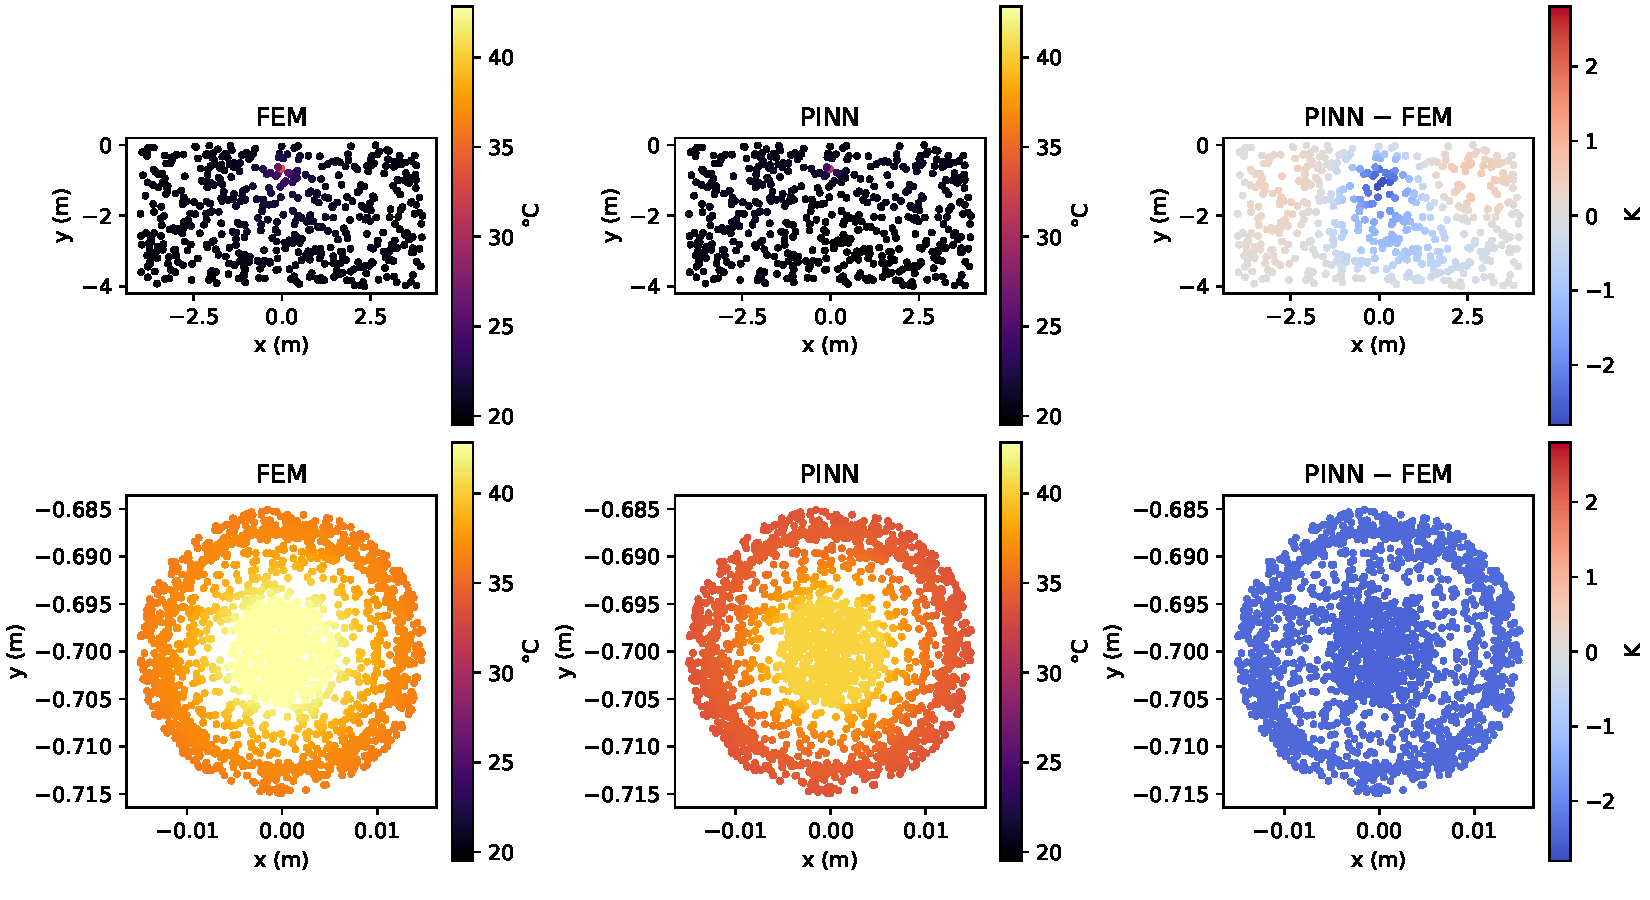
\includegraphics[width=\textwidth]{explicit/field.pdf}

\caption{Suelo y detalle interior del cable en XLPE con zona seca cercana, semilla 71 fijada previamente. Las temperaturas comparten escala y el error usa escala simétrica. Fuente: campos de confirmación.}\end{figure}
